%!TEX root = ../Report.tex

In this chapter, we will detail the current approaches to parallel programming. We will then explore the three key ideas requisite to this project, such that we can discuss how they are combined and the implications.

The main new idea in this project is that of dynamic contention aware scheduling. It has been shown to be an important factor in multiprogramming systems with performance implications (cite LIRA). Plasticity is a technique to respond to this challenge, and take it further. This results in complex code, making it hard to ensure correctness. So we use skeletons to abstract this complexity away from the programmer. It also has the nice side effect of dividing the challenge into a pattern-by-pattern basis.

In this project we will produce such skeletons, and investigate the performance implications of these ideas, as it is not known whether they will have a significant effect.



\section{Current Solutions}

Current solutions for parallel programming include:

\begin{itemize}
	\item Pthreads (POSIX Threads)
	\item MPI 	   (Message Passing Interface)
	\item OpenMP   (Open Multi-Processing)
\end{itemize}

These are the more conventional methods of parallel programming.

Pthreads provides the highest level of fine grain control, leaving most of the work to the programmer. As such, some parallel processing techniques may only be possible with Pthreads. It is implemented in the POSIX library, and is well integrated with the standard GNU compiler collection (\textbf{gcc}). Pthreads only makes sense with a shared memory architectures.

MPI is a communication library, and as such mostly details how processes can communicate. It is the dominant model used in the high performance computing industry today (cite https://dl.acm.org/citation.cfm?id=1188565). It can not only be used for a parallel program running on a single machine, but can also be used to implement a parallel program running on a distributed memory system.

OpenMP is comprised of compiler directives, runtime library routines, and environment variables. It is mostly used for loop parallelization, and is much higher level. It is also not limited to C.Like Pthreads, OpenMP is intended for shared memory architecture as it is thread bound.

Each of these methods have their own way of dealing with the complications introduced with parallel programming, which range from race conditions to limited scalability. These new problems can certainly be overwhelming to a traditionally sequential application programmer, so much so that there is entire books dedicated to the use of each of these particular parallel programming methods. 



\section{What Is Contention Aware Scheduling?}

It is known that in multiprogramming systems, with many programs running simultaneously, the choice of program to socket mapping significantly affects the performance of the system. (cite LIRA Section 2: Motivating Example) In the cite'd(?) case, just considering two programs running on the same socket, we can see from the graph in figure 2 (Cite) that certain programs perform differently with others, with some strange cases where the programs actually display better performance when running in contention with another. This problem is called co-scheduling.

So with this evidence, we can see that if we take into account these factors in our scheduler, we may obtain better overall performance. The outcome of the LIRA paper concludes that throughput gains of 3-7\% can be seen. Socket/resource aware scheduling in this manner is called a contention aware scheduler. Adding in the plastic programming idea could make this particularly powerful, because we know and control the specifics of the implementations, and not only can we control what program runs where, we can also adjust the implementation the program is using.



\section{What Is Plastic Programming?}

When programming an algorithm, there are often many choices about the specific implementation which can greatly affect performance, and the best choice depends on the circumstances of the problem. We tend to have more choices with parallel programs, but this is the case even for sequential programs. As an example, for a sorting problem with a large input size, radix sort would perform best, whereas for a small input size, insertion sort would be better. So naturally, in the interests of performance, we can conceive of a better overall implementation by combining the two approaches, so while the task size is large we would use radix sort, and then once it is reduced we would use insertion sort. An example of this can be seen in figure \ref{fig:plastic_graph}. 

(***Should the figure explanation be here or in the figure caption or both?***)

Such compositions are commonplace, such as the sorting example discussed in the PetaBricks paper (cite PetaBricks: Introduction, paragraph 2). Compared to PetaBricks, our implementation of plastic programming will be a little different. With the PetaBricks system, the programmer must specify multiple implementations for the compiler to switch between. In our system, we provide the various implementations, meaning no extra effort is required from the programmer.



\begin{figure}
	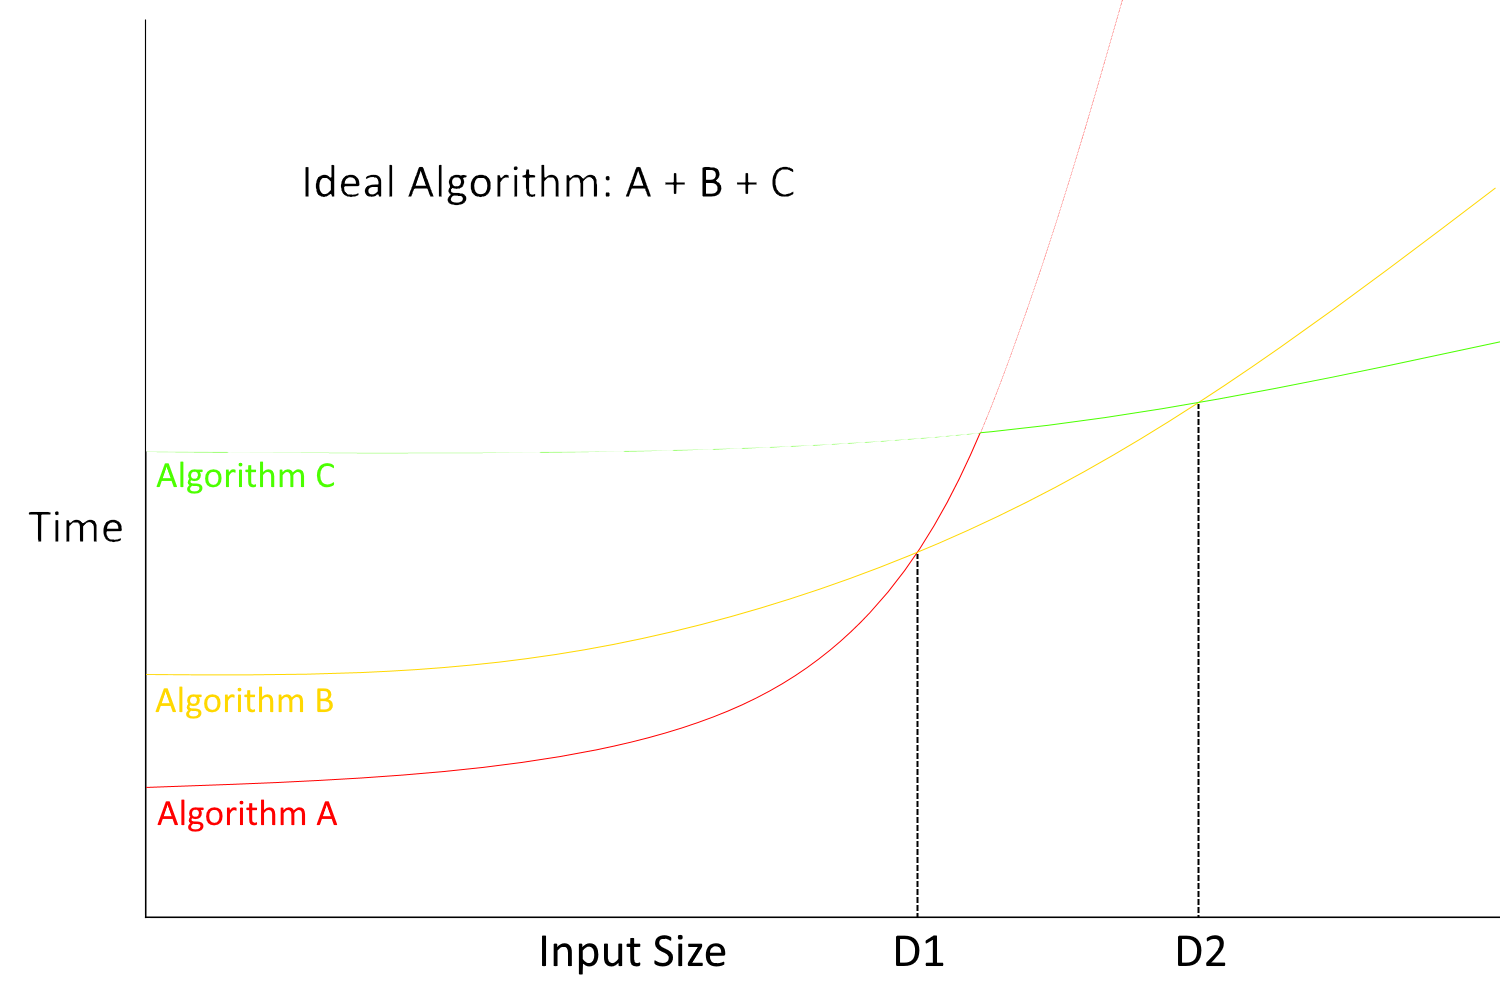
\includegraphics[width=\textwidth]{plastic_graph}
	\caption{An graph showing three algorithms with different runtime curves, which depend upon the array size. Combining these algorithms would provide an improved algorithm, with D1 and D2 showing the optimal decision points where a plastic programming system should switch algorithms}
	\label{fig:plastic_graph}
\end{figure}



\section{What Is Skeleton Programming?}
\label{section:background_skeleton_programming}

Skeleton programming is a high-level programming model. Skeletons will allow us to abstract away all the complexity involved in parallel programming, plastic programming, and co-scheduling. The essence of skeleton programming is that the skeleton provides the core structure of an algorithm, the user provides some code (In our case, a function), which then produces a correct program for the task at hand. The skeleton handles the hard-work of providing and optimizing the code (In our case, dealing with parallelism, plasticity, and co-scheduling). Possibly the most common skeleton is map, which is a skeleton that takes a function, an array of data, and applies the function to each member of the array. 

The consequences of this are twofold:

\begin{itemize}
	\item Errors are reduced substantially, as parallel programming is not easy, even without plasticity and contention aware scheduling.
	\item We can assess the program's complexity, since we know the algorithmic details of the skeleton.
\end{itemize}

Typically, multiple skeletons are combined to produce a more complex program, for example, a common combination is Map and Reduce. The ability to combine skeletons makes them a powerful tool, allowing programmers to easily create clean complex programs.

% There do exist? Doesn't sound quite right.

There does exist attempts to make parallel programming simple utilizing skeletons These include:

\begin{itemize}
	\item SkePU
	\item The Münster Skeleton Library Muesli
\end{itemize}

These methods simplify the problem, with both utilizing skeleton programming to do so. Since each SkePU skeleton has multiple implementations, and SkePU automatically selects the expected fastest implementation variant, it is the closest to the system we wish to implement.



\section{Summary}

In this chapter, we described the three fundamental concepts behind this project, contention aware scheduling, plastic programming, and skeleton programming. With just contention aware scheduling, we can achieve greater performance (cite LIRA). In this project we will take this idea further, adding plastic programming, so we can adapt the implementation of programs at runtime. This lets us change the implementations to ones which we know work well together. Combining these two ideas results in considerable complexity, so to make it simple for a programmer to use and easier for us to program, we use skeletons to abstract this complexity. The details of this complexity and how these ideas are combined are described in chapter \ref{chapter:implementation}.

The intent of this project is to explore the extent to which this approach can outperform a contention aware scheduled system which doesn't utilize plasticity.